\documentclass[a4paper]{article}
\renewcommand{\rmdefault}{ftm}
\usepackage[14pt]{extsizes}
\usepackage[utf8]{inputenc}
\usepackage[russian]{babel}
\usepackage{graphicx}
\usepackage{setspace,amsmath}
\usepackage[left=25mm, top=15mm, right=10mm, bottom=25mm, nohead, footskip=10mm]{geometry}
\begin{document}
\begin{center}
\hfill \break
\large{\textbf{ФГБОУ ВО«Московский Политехнический университет»}}\\
\hfill \break
\hfill \break
\hfill \break
\hfill \break
\hfill \break
\hfill \break
\hfill \break
\large{Лабораторная работа№2}\\
\footnotesize{Линейные программы\\
Задание 1,2,3\hspace{3cm}Вариант№1\break\\
По дисциплине:\\
Основы Программирования
}
\end{center}
\hfill \break
\hfill \break
\hfill \break
\hfill \break
\hfill \break
\hfill \break
\hfill \break
\hfill \break
\hfill \break
\hfill \break
\normalsize{ 
\begin{tabular}{ccc}
\hspace{4cm}Выполнил & Шукуров Ф.Ф  & группа 181-362\\
\\
\hspace{4cm}Проверил & \underline{\hspace{3cm}}& Никишина И.Н
\end{tabular}
}
\hfill \break
\hfill \break
\hfill \break
\hfill \break
\hfill \break
\hfill \break
\hfill \break
\hfill \break
\hfill \break
\hfill \break
\hfill \break
\hfill \break
\begin{center}\texttt{Москва 2018}\end{center}
\thispagestyle{empty}
\newpage
Лабораторная работа№2.27
\\
\begin{center}Задание№1\end{center}
    \begin{lab1}
       Постановка задания: Написать программу которая по заданному значению аргумента вычисляет значение функции, заданной в виде графика:
        \begin{center}
            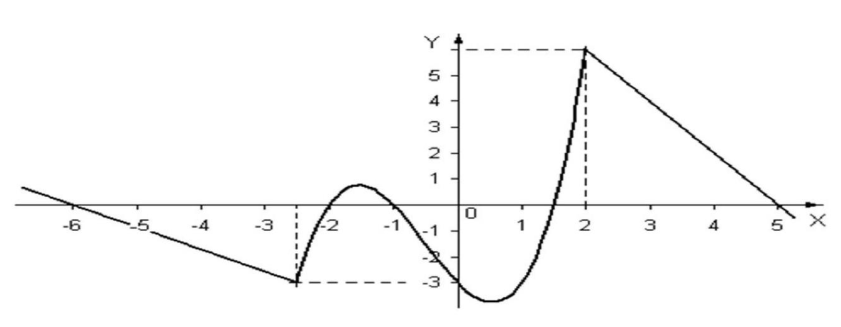
\includegraphics[width=\textwidth]{BOP/for_lab_1.png}
        \end{center}
    \begin{theory}
        Теоретическая часть:
        Для решения данной задачи были использованны блоки исключения
        \begin{verbatim}
            if<логическое выражение>:
                <блок выполняется при истинном выражении>
            elif<логическое выражение>:
                <блок выполняется при истинном выражении>
        \end{verbatim}
    \end{theory}
    \begin{description}
        Описание программы:\\
        Программа была написана на алгоритмическом языке python v3.6, реализованна в среде os Linux, и состоит из блоков ввода, проверки информации и вывода результата.
    \end{description}
    \begin{algoritm}
        Описание Алгоритма:
        \small\begin{enumerate}
            \item Ввод данных с клавиатуры
            \item Решение задачи, нахождение уравнений, а так же ОДЗ.
            \item Отталкиваясь от полученного результата, создать блоки исключений
            \item Добавить проверку на коректность ввода
            \item Вывод результата
        \end{enumerate}
    \end{algoritm}
        \texttt{Листинг Программы:}
    \begin{verbatim}
from math import *
import math
try:
    x = int(input("Введите значние X: \n"))
    if x <=-2.5: y = -6/7*x-36/7
    elif -2.5<x and x<2: y = x**3 + 1.5*x**2-2.5*x-3
    elif 2<=x: y = -2*x + 10
    print("X={0:.2f}   Y={1:.2f}".format(x,y))
except:
    print('Ошибка ввода.')
    \end{verbatim}
    \begin{center}
    Результат работы программы:
        \begin{verbatim}
            Введите значние X: 21
            X=21.00   Y=-32.00
            Введите значние X: 4
            X=4.00   Y=2.00
            Введите значние X: 2
            X=2.00   Y=6.00
        \end{verbatim}
    \end{center}
    \end{lab1}
    \begin{thebibliography}{}
    \bibitem{Список литературы: }
        https://www.pythonforbeginners.com/error-handling/python-try-and-except
        \item Майкл Доусон <<программируем на python>>
    \end{thebibliography}
\hfill\break

\begin{center}\underline{\hspace{5cm}}\\Задание№2\end{center}
\\
    \begin{lab2.2}
        Постановака задания: Написать программу, которая определеяет, попадает ли точка с заданными координатами в заштрихованную область.
    \begin{introduction}
        \begin{center}
            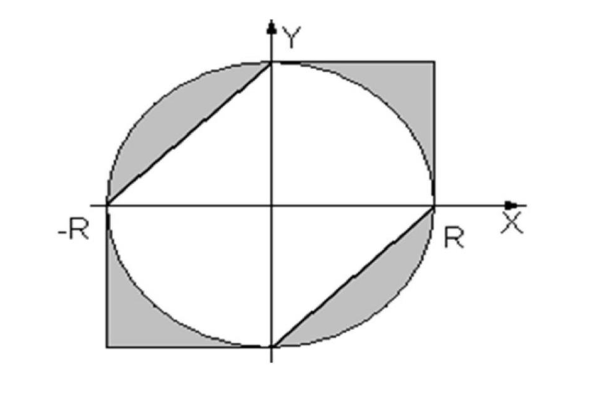
\includegraphics[width=100mm,scale=0.5]{BOP/for_lab_2_last.png}
        \end{center}
    \end{introduction}
    \begin{description}
        Описание программы:
        Программа находит по заданным значениям X, Y и R
    \end{description}
    \begin{algoritm}
        Описание Алгоритма:
        \small\begin{enumerate}
            \item Для начала определим в какой четверти находится точка заданная пользовательским вводом 
            \item Находим радус данной точки по теореме пифагора $C=\sqrt{A{^2}+B{^2}}$ где <<C>>~--- Радиус от(0;0)
            \item Если точка находится в II или IV четверти оси координат, и радиус данной точки \texttt{не превышает} радиус введенного пользователем, а так же результат уравнения прямой заданного вида <<y >||< x-RADIUS>> является истинной, то вывод информации о принадлежности точки к области
            \item Если точка находится в III или I четверти оси координат, и радиус данной точки \texttt{превышает} радиус введеного пользователем, а так же результат уравнения прямой заданного вида <<y >||< -x-RADIUS>> является истинной, то вывод информации о принадлежности точки к области
            \item Проверка ввода на корректность c помощью блоков Try:$>>>$ Exceptr:
        \end{enumerate}
    \end{algoritm}
        \texttt{Листинг Программы:}
    \begin{verbatim}
def two_four():
    if x>0 and y<0 and y<x-RADUIS:
        true()
    elif (x<0 and y>0) and y>x+RADUIS:
        true()
    else:
        error()
def error():
    print('Точка не принадлежит области')
def true():
    print('Точка принадлежит области')
def one_three():
    if x<0 and y<0 and y<-x-RADUIS:
        true()
    elif x>0 and y>0 and y>-x-RADUIS:
        true()
    else:
        error()
try:
    RADUIS = int(input('Введите радиус: \n'))
    x = int(input('Введите значение X: \n'))
    y = int(input('Введите значение Y: \n'))
    po_r = sqrt(x**2+y**2)  # point_radius
    if math.fabs(x)<=RADUIS and math.fabs(y)<=RADUIS:
        if po_r<=RADUIS:
            if (x<0 and y>0) or (y<0 and x>0): #первая и четвертая 
                                               #четверть
                two_four()
            else:
                error()
        elif po_r>=RADUIS:
            if (y>0 and x>0) or (x<0 and y<0):
                one_three()
            else:
                error()
        else:
            error()
    else:
        print('Точка находится вне графика')
except:
    print('404!')
    \end{verbatim}
    \end{lab2.2}
\end{document}
